\documentclass[a4paper, 12pt]{article}

\usepackage{fancyhdr}
\pagestyle{fancy}
\lhead{PROJET : Forteresse}
\lfoot{Info Sup}
\rfoot{EPITA 2016}
\renewcommand{\footrulewidth}{0.3mm}

\usepackage[french]{babel}
\usepackage{listings}
\usepackage[T1]{fontenc}
\usepackage{eurosym}

\usepackage[utf8]{inputenc}
\usepackage{graphicx}


\begin{document}
\begin{titlepage}
  \begin{sffamily}
  \begin{center}

    % Upper part of the page. The '~' is needed because \\
    % only works if a paragraph has started.

    \textsc{\Huge Cahier des charges}\\[3cm]

    \textsc{\LARGE Projet:}\\[1.5cm]

    % Title
	\centerline{
\includegraphics{coollogo_com-19602433.png}}
	\vfill{
	\centerline{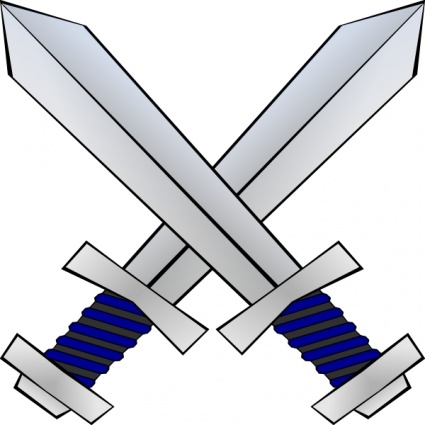
\includegraphics[scale=0.4]{crossed-swords-clip-art-48219.jpg}}}

    % Author and supervisor
    \begin{minipage}{0.4\textwidth}
      \begin{flushleft} \large	
      
      \end{flushleft}
    \end{minipage}
	\begin{flushleft}\vfill
      {
       \textsc{Chatelus} Florian\\
       \textsc{Henric} Arnaud\\
       \textsc{Sarkar} Riday\\
       \textsc{Ezzahoui} Yassine }
    \end{flushleft}	
  \end{center}
  \end{sffamily}
\end{titlepage}
\tableofcontents
\newpage
\section{Introduction}
Ce cahier des charges a pour but de vous présenter le projet que nous allons réaliser durant le deuxième semestre de notre année de Sup . Dans ce cahier des charges vous aurez accès aux différentes étapes du développement de notre jeu ainsi que les moyens humains et matériels mis en oeuvre dans la réalisation du projet.
Forteresse est en fait un tower defense issu de l’imagination de Henric Arnaud, Sarkar Riday,Chatelus Florian et de Ezzahoui Yassine.
Nous établirons un planning dans lequel chaque membre aura un but précis à accomplir pendant une durée déterminée.
Ce cahier des charges contient également un planning détaillé qui servira à mettre en avant  la réalisation des différentes parties du jeu afin que celui-ci soit terminé le 20 juin.
Ainsi vous allez  apprendre  dans ce cahier tout ce que vous avez besoin de savoir concernant de la réalisation de ce projet : présentation, découpage du projet et organisation de la réalisation.
La motivation principal est  d’ obtenir un jeu fonctionnel qui correspond aux attentes  et aux ambitions de chacun.


\section{Présentation}
	\subsection{Les membres du groupe}
	\parindent=0cm\textbf{Florian \textsc{Chatelus}}
	\smallbreak
	\par \parindent=0.5cm Commence enfin l'une des raisons pour laquelle j'ai choisi l'EPITA, le projet! A mon arrivé a l'EPITA la programmation ne m'était pas totalement inconnue puisque j'ai eu la chance de pouvoir choisir la spécialisation ISN en Terminale. Nous avions réussi avec mon groupe a recréer le célèbre PONG. Bien que mon projet d'ISN ai été très basique, je pense qu'il me servira au moins dans les démarches de réalisation du projet. J'ai donc une petite expérience en ce qui concerne le travail de groupe, que j'espère arriver a mettre a profit pour notre projet de cette année. Malgré tout, ce projet sera un réel challenge pour moi, puisqu'il nous obligera a faire appel a de nombreuse compétence que nous ne disposons pas encore. Ce sera donc un formidable exercice, qui demandera une certaine rigueur dans le travail certes, mais qui me permettra de progresser rapidement.\\
	
	\parindent=0cm\textbf{Arnaud \textsc{Henric}}
	\smallbreak
	Le projet de première année, enfin ! Nous avons déjà eu des TPs de programmation mais le projet permettra de nous tester d’avantage. En groupe, nous allons réaliser un devoir que nous avons nous-mêmes choisi, un jeu-vidéo. J’ai déjà réaliser certains projets en ISN au lycée (le triangle de Sierpinski, le jeu de la vie ou encore un code barre) mais jamais de projet comme celui-ci, sur un semestre entier et en groupe. Néanmoins ISN m’a donné un peu d'expérience et je suis prêt à créer ce jeu vidéo.\\
	
	\parindent=0cm\textbf{Riday \textsc{Sarkar}}
	\smallbreak
 Avant d’arriver à EPITA,  j'ai jamais touché à une ligne de code a part cliquer de temps en temps sur des icônes avec Algobox en cours de maths (au passage c'était très bien pour découvrir  le monde merveilleux de l’algorithmique). Je suis conscient que réaliser les tâches qu’on m’a données ne sera pas facile. Cela étant dit, je sais que ce projet est un plus pour nous et qu’on va apprendre beaucoup de choses à travers la réalisation de ce projet. Donc je vais jouer le jeu et faire un maximum de choses pour le projet et essayer d’apprendre un maximum de choses à travers la réalisation de ce projet.\\

	\parindent=0cm\textbf{Yassine \textsc{Ezzahoui}}
	\smallbreak
	Nous abordons  le projet de première année avec ambition et envie , nombreux seront les défis à relever . Pour ma part avant cette année je n’avais aucune notion en programmation , ce projet me permettra donc d’apprendre différents langage de programmation ,  de connaître tous les paramètres qui régissent un travail de groupe de cette ampleur. Ainsi ce  projet est pour moi  un atout pour l’apprentissage de tout les aspects que peut m’offrir la programmation .

	\parindent=0.5cm 
	\subsection{Les origines du projet}
Nous avons choisi de réaliser un jeu plutôt qu’un logiciel car nous avons deux membres dans le groupe qui ont déjà réalisé un jeu en Terminale dans le cadre d’un projet en groupe. Même si le projet achevé en ISN par ces deux derniers n’est pas comparable avec ce qui nous attend ce semestre en INFO SUP, ce sera toujours une aide non-négligeable.
\par Une fois que la nature du projet était choisi, nous avons réfléchi longuement sur le type de jeu que nous allons réaliser. Notre expérience en tant que joueur nous donnait un large choix parmi les types de jeu possibles comme un RPG (Role Playing Game), RTS (Real Time Strategy) ou encore un Tower Defense . 

	\subsection{Le jeu}
		\subsubsection{Présentation}
		\par Notre jeu sera basé sur le principe du \textit{tower defense}. Qu'est-ce que 			cela signifie? Un \textit{tower defense}, est un jeu qui comme son nom l'indique 			aura comme objectif de défendre un point donné. Le but du jeu sera donc de défendre 		un cristal qui alimente la porte de l'endroit que nous souhaitons protéger.  
		\subsubsection{Déroulement d'une partie}
		Une partie se déroulera en deux phases qui se répéteront, a chaque vague d'ennemis.\\
		\centerline{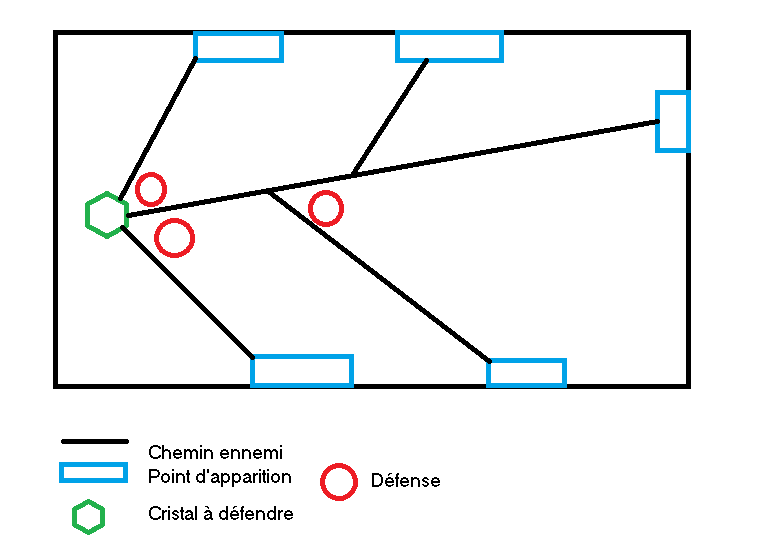
\includegraphics[scale=0.55]{Plan.png}}
		\par La première est la phase que nous appellerons \textit{phase de préparation}, elle consiste à préparer ses défenses, en les positionnant de façon stratégique, les améliorant ou en les réparant. Cette phase sera d'une importance capital pour assurer une victoire lors de la phase suivante. Une fois que vous serez fin prêt pour le combat, il vous suffira d'appuyer sur prêt et la deuxième phase commencera une fois tout les joueurs prêt.
		\par Nous arrivons donc en deuxième phase, la \textit{phase de combat}, qui va déclencher l'action. Des créatures vont apparaitre à des points précis de la carte et vont converger vers le ou les cristaux. Le joueur pourra donc durant cette phase attaquer les monstres et tenter de les détruire et/ou continuer à poser, améliorer et réparer ses constructions mais avec des malus d'incantation.
		\par Tous les certains nombre de cycle, au terme de ces deux phases, un monstre plus imposant apparaitra, et le joueur devra s'en défaire afin de remporter la manque et d'obtenir des objets.
		\subsubsection{L'interface}
		L’interface permettra au joueur d'être renseignée à tout moment sur : 
		\begin{itemize}
		\item Le temps écoulé.
		\item Sa jauge de vie.
		\item L’arme dont il est en possession , ainsi que les  munitions dont il dispose.
		\item L’argent qu’il possède pour acheter de nouvelles tours ou armes.
		\end{itemize}
		\subsubsection{L'arsenal de défense}
		Nous utiliserons donc différents types d’armes de type médiéval fantastique.
Les armes seront donc accessible en la ramassant sur un bosse ou bien  suite à un achat du joueur, elles pourront être améliorer, durant la partie. On distinguera plusieurs types d’armes tel que:
	\begin{itemize}
	\item Les épées.
	\item Les arcs.
	\item Les bâtons.
	\end{itemize}
Les défenses fixes seront achetable grâce a l’argent gagné durant la partie. Les défenses seront comme les armes améliorables. Ces dernières seront autonomes et feront partie de l’IA. On pourra y trouver:
	\begin{itemize}
	\item Des tourelles.
	\item Des pièges.
	\item Des auras.
	\end{itemize}
\section{Découpage du projet}
	\subsection{Le graphisme}
		\subsubsection{La 3D}
		Étant donné sa gratuité, nous allons utiliser Blender pour réaliser des modèles 3D. Ce logiciel va nous permettre de modéliser les différents personnages de notre jeu et de faire les diverses textures de l’environnement du jeu.

		\subsubsection{La 2D}
		La 2D de notre jeu sera principalement représenté par l'interface graphique du joueur. En effet, le joueur aura besoin d'avoir des informations et de repère visuel afin d'interagir correctement avec son environnement et d'avoir une expérience de jeu la meilleure possible. La 2D pourra également jouer un rôle important dans les menus.
	\subsection{Audio}
	L’audio gère évidemment tous les sons. De bruitages dans le jeu à musique dans les menus, nous devrons trouver des sons qui s’adaptent au contexte médiéval.

	\subsection{Le réseau}
	Le réseau consistera tout simplement a implémenter un mode multijoueur, afin que les joueurs puissent jouer ensemble en ligne ou bien en réseau local.
	\subsection{L'intelligence artificiel}
	Pour définir l’IA, nous allons créer différents niveaux de difficultés. Le but est que l’IA détruise le cristal que nous devons protéger, ainsi, l’IA est l’ennemie. Il contrôle plusieurs personnages. Nous devons coder un IA capable de se déplacer vers le cristal, mais également de combattre contre l’utilisateur, de mourir tué par le héros ou les tourelles. 

	\subsection{Le menu}
	Nous tenterons de créer un menu accessible et design. Il devra permettre d'accéder au lancement d’une nouvelle partie, aux options, ainsi qu’au mode multi-joueur. 
	\subsection{Le site}
	Modéliser un site web avec une présentation générale des créateurs et de la création (chronologie, problèmes, solutions…). Ajouter des images du jeu. Expliquer les règles.  Donner les références utiles pour notre réalisation. Permettre le téléchargement du jeu aux utilisateurs, et mettre à disposition le rapport ainsi que le jeu en version lite.
	\subsection{Gameplay}
	Le gameplay consiste à coder tous les mouvements de notre héros, soit le personnage que l’on contrôle… Il devra être capable de donner des coups, construire des tours, courir, sauter, et bien sûr, se déplacer à n’importe quel point accessible de la map. Le gameplay consiste également à coder la caméra suivant notre héros. Ce jeu se jouant à la troisième personne, la caméra devra être capable de toujours regarder le héros de derrière et de le suivre dans tous ses mouvements. On devra ici géré également tous les problèmes de collision.
	\subsection{Animation}
	L’animation est le moyen de rendre les mouvements des personnages fluides et réalistes. Chaque mouvement devra être animé, les jambes lorsqu’un personnage se déplace, les bras lorsqu’il combat, etc...



\section{Répartition des tâches}
Nous avons décidé d’attribuer chaque tâche à au moins deux personnes car ainsi chaque membre réalise plusieurs tâches et peut apprendre des choses de domaines différents . De plus, si un membre rencontre des difficultés et se retrouve bloqué pour réaliser une tâche, son coéquipier peut venir en aide puisqu’ils s’occupent de la même tâche. Ainsi la réalisation des tâches devient plus facile.
\bigbreak
\bigbreak
	\begin{tabular}{|c||c|c|c|c|c|}
		\hline
		& Florian & Riday & Yassine & Arnaud \\
		\hline
		Site & & & $\times$ & $\times$\\
		\hline
		3D & & $\times$ & $\times$ &\\
		\hline
		2D & $\times$ & $\times$ & $\times$ & $\times$ \\
		\hline
		IA & $\times$ & & & $\times$\\
		\hline
		Multijoueur/Réseau & $\times$ & $\times$ & $\times$ & $\times$\\
		\hline
		Menu & & & $\times$ & $\times$\\
		\hline
		Gameplay & $\times$ & $\times$ & &\\
		\hline
		Animation & & $\times$ & & $\times$\\		
		\hline
		Audio & $\times$ & & $\times$ &\\
		\hline
		\LaTeX & $\times$ & $\times$ & &\\
		\hline
	\end{tabular}
	\newpage
\section{Ressources utilisées}
	\subsection{Ordinateur}
	Nous utiliserons a l'évidence des ordinateurs. Ils seront notre principal outil de travail. Nous utiliserons un ordinateur dans toutes les étapes de notre projet. 
	\subsection{Visual Studio 2015}
	Visual Studio est le logiciel qui nous permettra de coder nos scripts sur Unity. Nous l'utiliserons plus particulièrement afin d'utiliser le langage C\# qui représentera la quasi-totalité, voir la totalité de notre code.
	\subsection{Unity}
	Unity sera LE logiciel cœur de notre projet, il lui servira de base. Il nous permettra de mettre en relation des objets avec des scripts que ces objets effectuerons. Ce logiciel correspond parfaitement a nos besoins, dans la réalisation d'un jeu vidéo. De plus il possède une courbe d'apprentissage linaire et est facile d'accès, ce qui correspond à nouveau avec notre statut d'étudiant en première année.
	\subsection{Gimp/Blender}
	Gimp est un éditeur graphique. Il nous sera utile notamment pour la création de la 2D, et donc de l'interface graphique de notre jeu. Sans oublier la jaquette de notre jeu lorsqu'il sera en version CD.
	\par Blender quant a lui est un logiciel de modélisation 3D et sera simplement destiné a la création d'éléments 3D pour notre jeu. 
	\subsection{Tutoriel}
	Enfin, la ressource que nous utiliserons le plus, après nos ordinateurs, sont les tutoriels. Dans la mesure où, cette expérience est inédite pour chacun d'entre nous, nous aurons besoin d'acquérir de nombreuses connaissances. C'est ici qu'interviendront les nombreux tutoriels à notre disposition sur le web. Notez que des tutoriels ont été visionné pour la réalisation de ce cahier des charges.
	\newpage
\section{Planning}
	\subsection{Première soutenance}
	\begin{tabular}{|c||c|c|c|c|}
		\hline
		& Non débuté & Débuté & Avancé & Terminé \\
		\hline
		Site & & & $\times$ & \\
		\hline
		3D & & $\times$ & &  \\
		\hline
		2D & & $\times$ & &  \\
		\hline
		IA & & $\times$ & &\\
		\hline
		Multijoueur/Réseau & & $\times$ & & \\
		\hline
		Menu & & & $\times$ & \\
		\hline
		Gameplay & & $\times$ & & \\
		\hline
		Animation & & $\times$ &  & \\		
		\hline
		Audio & $\times$ &  & &  \\
		\hline		
	\end{tabular}
	\subsection{Deuxième soutenance}
	\begin{tabular}{|c||c|c|c|c|}
		\hline
		& Non débuté & Débuté & Avancé & Terminé\\
		\hline
		Site & & & $\times$ & \\
		\hline
		3D & & & $\times$ & \\
		\hline
		2D & & & $\times$ & \\
		\hline
		IA & & $\times$ & & \\
		\hline
		Multijoueur/Réseau & & & $\times$ & \\
		\hline
		Menu & & & & $\times$\\
		\hline
		Gameplay & & $\times$ & & \\
		\hline
		Animation & & & $\times$ &\\		
		\hline
		Audio & & $\times$ & &\\
		\hline		
	\end{tabular}
	\subsection{Soutenance finale}
	\begin{tabular}{|c||c|c|c|c|}
		\hline
		& Non débuté & Débuté & Avancé & Terminé \\
		\hline
		Site & & & & $\times$ \\
		\hline
		3D & & & & $\times$ \\
		\hline
		2D & & & & $\times$ \\
		\hline
		IA & & & & $\times$ \\
		\hline
		Multijoueur/Réseau & & & & $\times$ \\
		\hline
		Menu & & & & $\times$ \\
		\hline
		Gameplay & & & & $\times$\\
		\hline
		Animation & & & & $\times$\\		
		\hline
		Audio & & & & $\times$ \\
		\hline		
	\end{tabular}
\section{Budget}

Nous sommes des étudiants et ceci est un projet de première année. C'est donc un projet dans le cadre scolaire et à but non lucratif. Ainsi, le budget sera de 0\euro{}. Aucun achat ne sera nécessaire à la réalisation de notre projet. Les dépenses seront donc également de 0\euro{}. Seul des logiciels gratuits ou bien fourni gratuitement par l'école seront utilisés dans ce projet. Un léger dépassement de budget est bien entendu possible, notamment pour l'achat d'un CD si cela s'avère nécessaire.\\
\centerline{
\includegraphics[scale=0.7]{images.jpg}}

\section{Conclusion}
Ainsi, Forteresse sera notre jeu-vidéo réalisé par Florian, Arnaud, Riday et Yassine (FARY). Situé dans un contexte médiéval, inspiré des conquêtes de l’époque, nous devrons à tout pris défendre notre cristal, attaqué par des ennemis aussi répugnants que menaçants. Pour cela, nos guerriers devront faire preuve de stratégie et de courage pour repousser les dangers. Capables de construire des tours de défense, ils devront les placer sur des lieux stratégiques afin de stopper l’invasion ennemie mais ils devront aussi user de leur force au combat.
Êtes vous capables de résister et de défendre vos cristaux ?
… à vous de jouer !!
\end{document}
